%
% Stimulus Overselectivity
%

\subsection{Lacking Appropriate Context}
Various contemporary theories hypothesize that people with autism possess deficits in integrating contextual information in an appropriate manner.  Problems integrating information, it is argued, result in a processing style which highlights the specific pieces of the environment at the cost of more general high-level information~\cite{HappeF:1999:WCC}. This ``piecemeal'' style is capable of explaining an impressive variety of both the advantageous and detrimental behavior demonstrated by people with autism.  One possible mechanism that could give rise to information integration difficulties would be a tendency to restrict attention to an excessively small number of features, with difficulty in shifting attention to other features.  In this section, we explore this possibility using a simple computational model of the role of prefrontal cortex in attention.

Stimulus overselectivity, where a restricted set of components within a compound stimulus tend to dominate behavior, was first documented in the early 1970s in people with autism~\cite{LovaasO:1971:Selective}.  This effect has since been demonstrated both within and across different modalities as well as by varying the number of features composing the compound stimulus~\cite{ReedP:2005:TaskLoad}.  The paradigmatic task involves conditioning responses to a stimulus made of multiple, simultaneously presented, components.  After the initial association of the compound stimulus with reward/response, each individual component is tested separately, assessing the degree each has acquired control over the subject's behavior. (See Figure~\ref{OS-Task}.)  Normally developing individuals respond equally to all components.  People with autism, to the contrary, are more likely to respond to a single component, thus demonstrating overselectivity.  Overselective behavior in people with autism is a plausible explanation for the observed problems in generalizing learned behaviors to novel situations.  In such situations, restricted, often irrelevant, portions of the environment become tightly coupled with the performance of the desired behavior.  If this restricted portion is not consistently available to the individual, generalization to new settings will suffer.  This is a major focus of many behavioral and intervention techniques. 

\subsection{Cognitive Flexibility \& Overselectivity}
Our modeling work on executive dysfunction demonstrates how impaired interactions between the mesolimbic dopamine (DA) system and the prefrontal cortex (PFC) can result in perseverative attention to an overly restricted set of stimulus dimensions and features, as exhibited by perseveration in the WCST~\cite{KrieteT:2015:ED}.  Utilizing an abstraction of this same mechanism, in the following we show how show how an analagous perseverative attention mechanism results in a significant increase in stimulus overselectivity.   

%An intriguing study suggests that stimulus overselectivity can be induced in healthy individuals by requiring the concurrent performance of a working memory task~\cite{ReedP:2005:TaskLoad} with overselectivity training consisting of learning a multi-component stimulus to response mapping.  Working memory tasks are widely believed to enlist the resources of PFC, providing additional support for the conjecture that healthy individuals utilize this area when performing this task.

\subsection{The Overselectivity Task}
An operant conditioning paradigm traditionally has been used when assessing the degree of overselective behavior in people with ASD.  In this psychological task, a compound stimulus, consisting of multiple separate components, is associated with an action that leads directly to reward.  The components can differ in modality (e.g. auditory, visual, and tactile) or be different stimuli within the same modality. After the initial stimulus / action / reward association has been learned, each individual component of the compound stimulus is presented separately in order to assess the degree each able to elicit a response.  The severity of overselective behavior is measured by noting the number of the compound components capable of eliciting a response in isolation from the others.  Overselectivity occurs when the number of components capable of driving a response in isolation is lower than the total number which comprise the compound stimuli.  If an individual responds to all components equally, this indicates that attention has been distributed across all components during learning and no overselectivity is demonstrated.   

\subsection{Modeling Overselectivity}
To investigate overselectivity, we utilized a simple artificial neural network model constructed using the biologically inspired Leabra framework~\cite{OReillyRC:2000:Computational}.   In this simple model (see Figure~\ref{network-diagram-2}), an input layer represents the components of the compound stimulus. It is useful to consider each unit of this layer as an individual component of a compound stimulus.  For example, the first three units can be thought of as representing an auditory, visual, and tactile component respectively.  To represent the compound, all three individual units are clamped to a high value simultaneously.  The Hidden layer learns stimulus to response mappings, and provides a modeled abstraction of posterior brain systems.  A response layer encodes the ``decision'' of the network based on information received from the computations performed within the network.  The two possible outputs represented within the response layer of the network are ``Respond'' and ``Do-Not-Respond''.  Importantly, a PFC layer provides a top-down influence on processing within the ``Hidden'' (posterior) layer.  The PFC layer has one extra unit which is utilized in the working memory load condition described below. (Note, however, that this working memory load unit is not shown in Figure~\ref{network-diagram-2}.).  The input layer also contains one extra unit, this unit can be thought of as representing a ``No Stimulus'' condition, analogous to when the participant is not being asked to respond to a stimulus object.  Each unit in the PFC layer is associated with exactly one unit in the input layer.  These input / PFC ``pairs'' project to a unique pool of hidden layer units, producing an isolated processing pathway for each stimulus component and its corresponding PFC unit.  This enables each individual PFC unit to have selective influence upon a unique individual component of the compound stimulus.  In other words, each hidden unit is directly modulated by only one of the three possible pathways.  Note, however, that there is full recurrence between all of the hidden layer units.  This does allow for one processing pathway to possibly influence the computations performed by another pathway.  Additionally, the unit representing the working memory load selectively projects to another isolated pool of hidden units.  These hidden units are also fully recurrent, and thus connected to all other hidden layer units as described previously.  Only one difference exists when comparing the working memory load unit to the other modeled PFC units and the unique processing pathways of which each is a part. Namely, the hidden units projected to by the working memory load unit do not receive any projections from the input layer.  This roughly corresponds to, and provides a way to model, the necessary lack of external stimuli during the performance of working memory tasks. 

\begin{figure}
\begin{center}
	\includegraphics[width=125mm]{figures/overselectivity_network.ps}
\end{center}
\caption{Network diagram of stimulus overselectivity model.} 
\label{network-diagram-2}
\end{figure}

When modeling both normal and autistic performance, the network learned to ``Respond'' to the compound stimulus by simultaneously activating the three appropriate input units, representing an auditory, tactile, and visual component respectively.  This is an extremely easy task for the network to learn, as it only needs to associate a response with the stimulus that is presented.  This duplicates the simplicity of the original behavioral study by Lovaas et al.  During the ``healthy'' normal condition, the PFC is allowed to switch between all three possible states, simulating a fully functional and flexible PFC.  When modeling autism, however, only a single unit of the PFC layer was activated, and remained so throughout the entirety of training.   Perseveration on the single PFC dimension simulates a deficit in flexibly updating the representations maintained within the PFC.  This difference, the ability to flexibly adapt representations actively maintained by the PFC, is the only parameter manipulated from the model of normal performance in order to simulate autistic-like performance, all other parameters remained constant between models.

After the initial stimulus / response training with the compound stimulus, each component was presented individually to the network.  The measure of interest is the number of individual components capable of correctly producing a ``Respond'' output from the network.  The results for simulated autistic and control performance are average results for 100 separate runs of the model in each condition.

One additional condition was tested within the model framework just described.  A recent study provides support for the role of PFC in overselective performance~\cite{ReedP:2005:TaskLoad}.  In this study, Reed et al. demonstrated that the addition of a working memory (WM) load, where additional items must be maintained and remembered at the end of a trial, actually leads to overselective responding in normally developing individuals.  This is interesting because WM tasks are traditionally associated with processes localized within the frontal lobes, which we argue is a vital cortical area involved in the development of overselectivity in people with autism.  In order to investigate whether our simple model can capture these results, an irrelevant additional item was maintained in the PFC layer during the initial learning phase, simulating a WM load.  This was achieved by keeping one ``extra'' PFC unit constantly actively throughout the entirety of training, simulating maintenance of extra information with the PFC.  All other parameters were identical to the ``Normal'' control condition.  This includes the flexible updating of the PFC, which  was allowed to flexibly switch between all three other items during training.

\subsection{Overselectvity Simulation Results}
My modeling efforts qualitatively match human performance and provide evidence that rapid and flexible updating of the PFC is necessary to prevent a restricted cue set from gaining control over behavior. (See Figure~\ref{OS-Model-Results-2}).  

\begin{figure}
\begin{center}
%	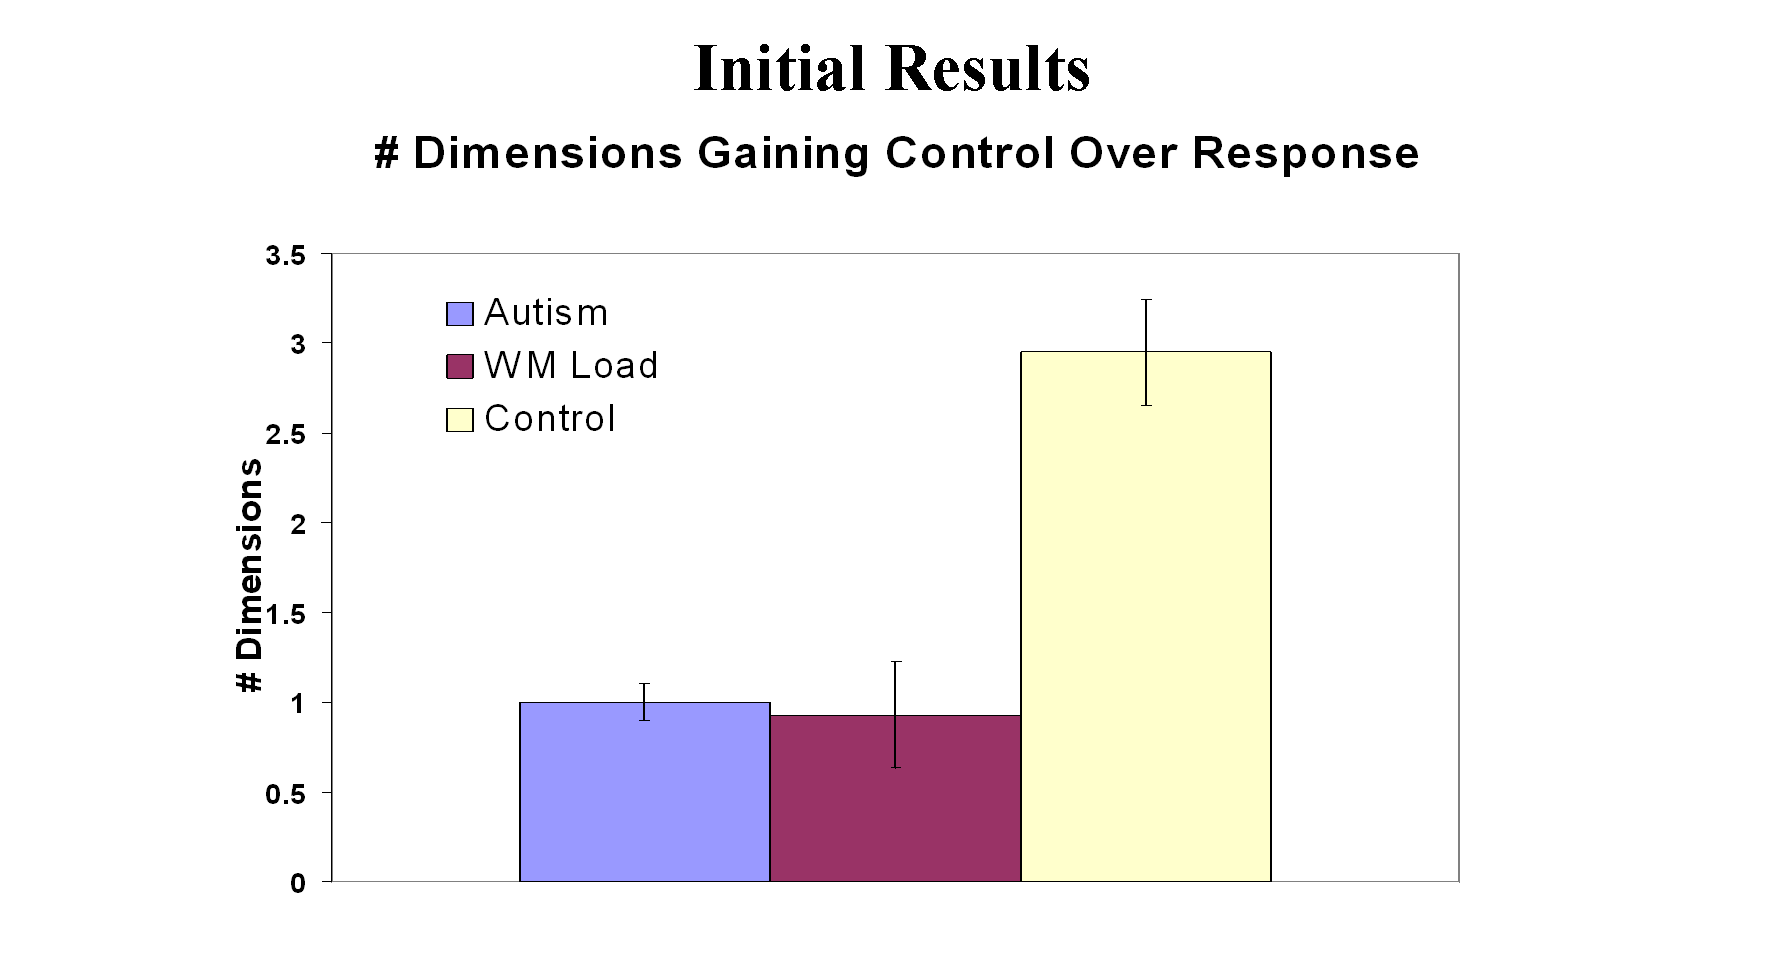
\includegraphics[width=125mm]{graphs/OS_initial_results.eps}
	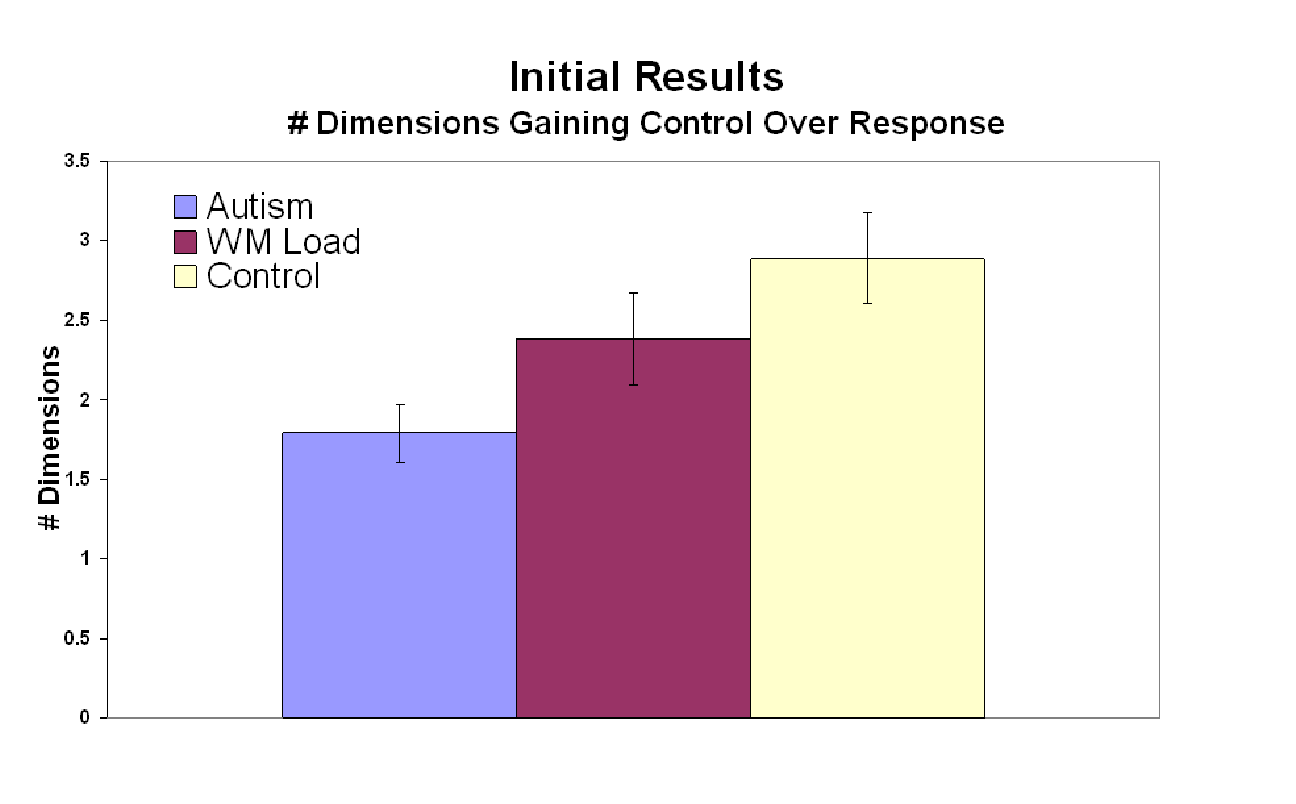
\includegraphics[width=125mm]{graphs/overselectivity_results_new.eps}
\end{center}
\caption{Simulation results modeling overselectivity task (see Figure~\ref{OS-Task}) by manipulating the flexible updating of a PFC-like mechanism. Only the simulation where the PFC is allowed to flexibly adjust the activation of its representations (``normal condition'') resulted in all three components of the compound stimulus gaining equal control over behavior.  Both the inflexible updating (autism condition) and the addition of irrelevant information in PFC manipulations (working memory load condition) result in a restricted subset of components gaining control over behavior, demonstrating overselective behavior.}
\label{OS-Model-Results-2}
\end{figure} 

The model of autistic performance responded to significantly fewer components ($p < .05$), compared to the model allowed to flexibly update its PFC representations, demonstrating overselective behavior.  Providing additional support for the hypothesis that the PFC influences learning in other cortical areas in interesting and important ways, a modeled WM load during training of a ``healthy'' network results in significantly more overselective responding ($p < .05$), also capturing recent behavioral results.  Overselectivity arises in this model due an effect of PFC-directed attention on the learning of associations between stimulus features and the response output.  When PFC activity is directed to a particular stimulus pathway, the activation levels of the hidden units of that pathway are increased.  Lateral inhibition within the Hidden Layer, driven by this increased activity, reduces activity in the pathways corresponding to the other stimulus components.  Thus, learning primarily takes place within the selected pathway, as synaptic plasticity is strongest in Leabra in the presence of presynaptic activity.  In the autism network, which remains focused on a single pathway throughout training, the synaptic weights grow strong only within the selected pathway, with the connections in the other pathways remaining relatively weak.  Thus, the autism network fails to learn to generate responses to the unattended stimulus features, even if attention is later directed to those features.  In contrast, the healthy model flexibly adjusts PFC activity during training, allowing different pathways to be strengthened on different trials, eventually producing strong associations between all of the stimulus features and the need to respond.  Leabra's Hebbian learning mechanism further ensures that these associations are robust. (See Figure~\ref{OS-Model-Cartoon}.)

\begin{figure}
\begin{center}
	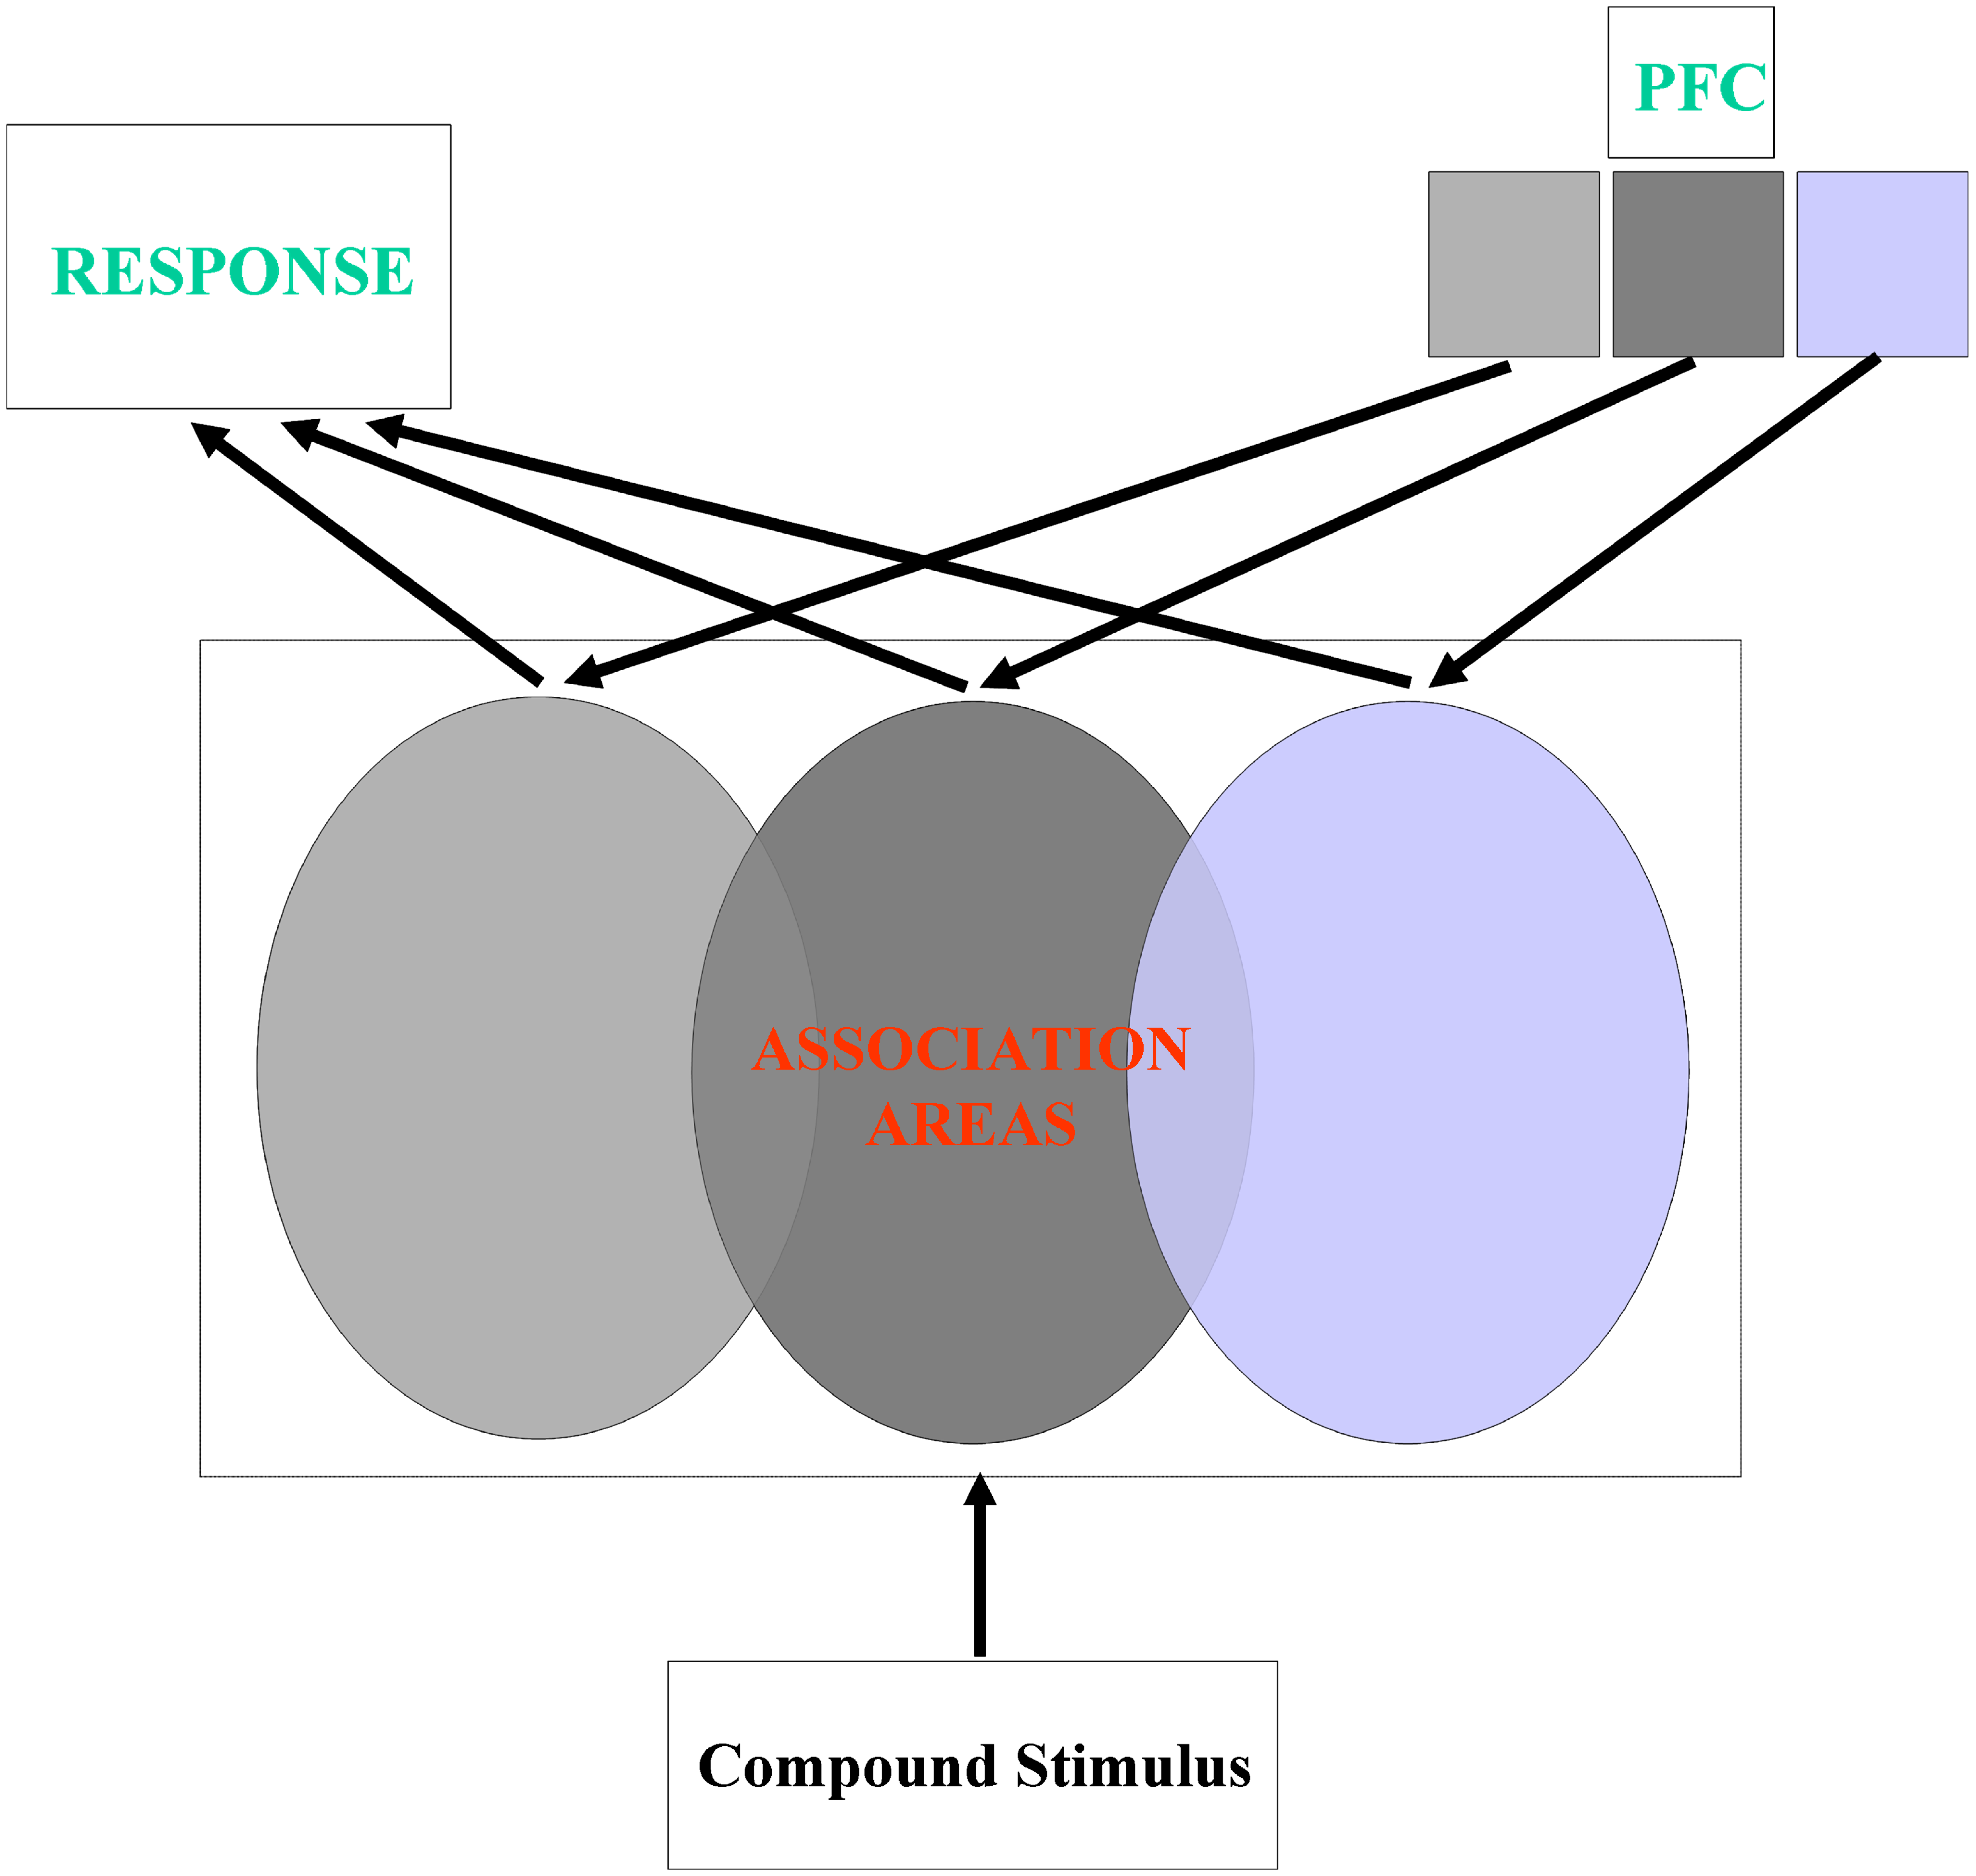
\includegraphics[width=70mm]{figures/so_model_no_persev_new_2.eps}

-----------------------------------------------------------

	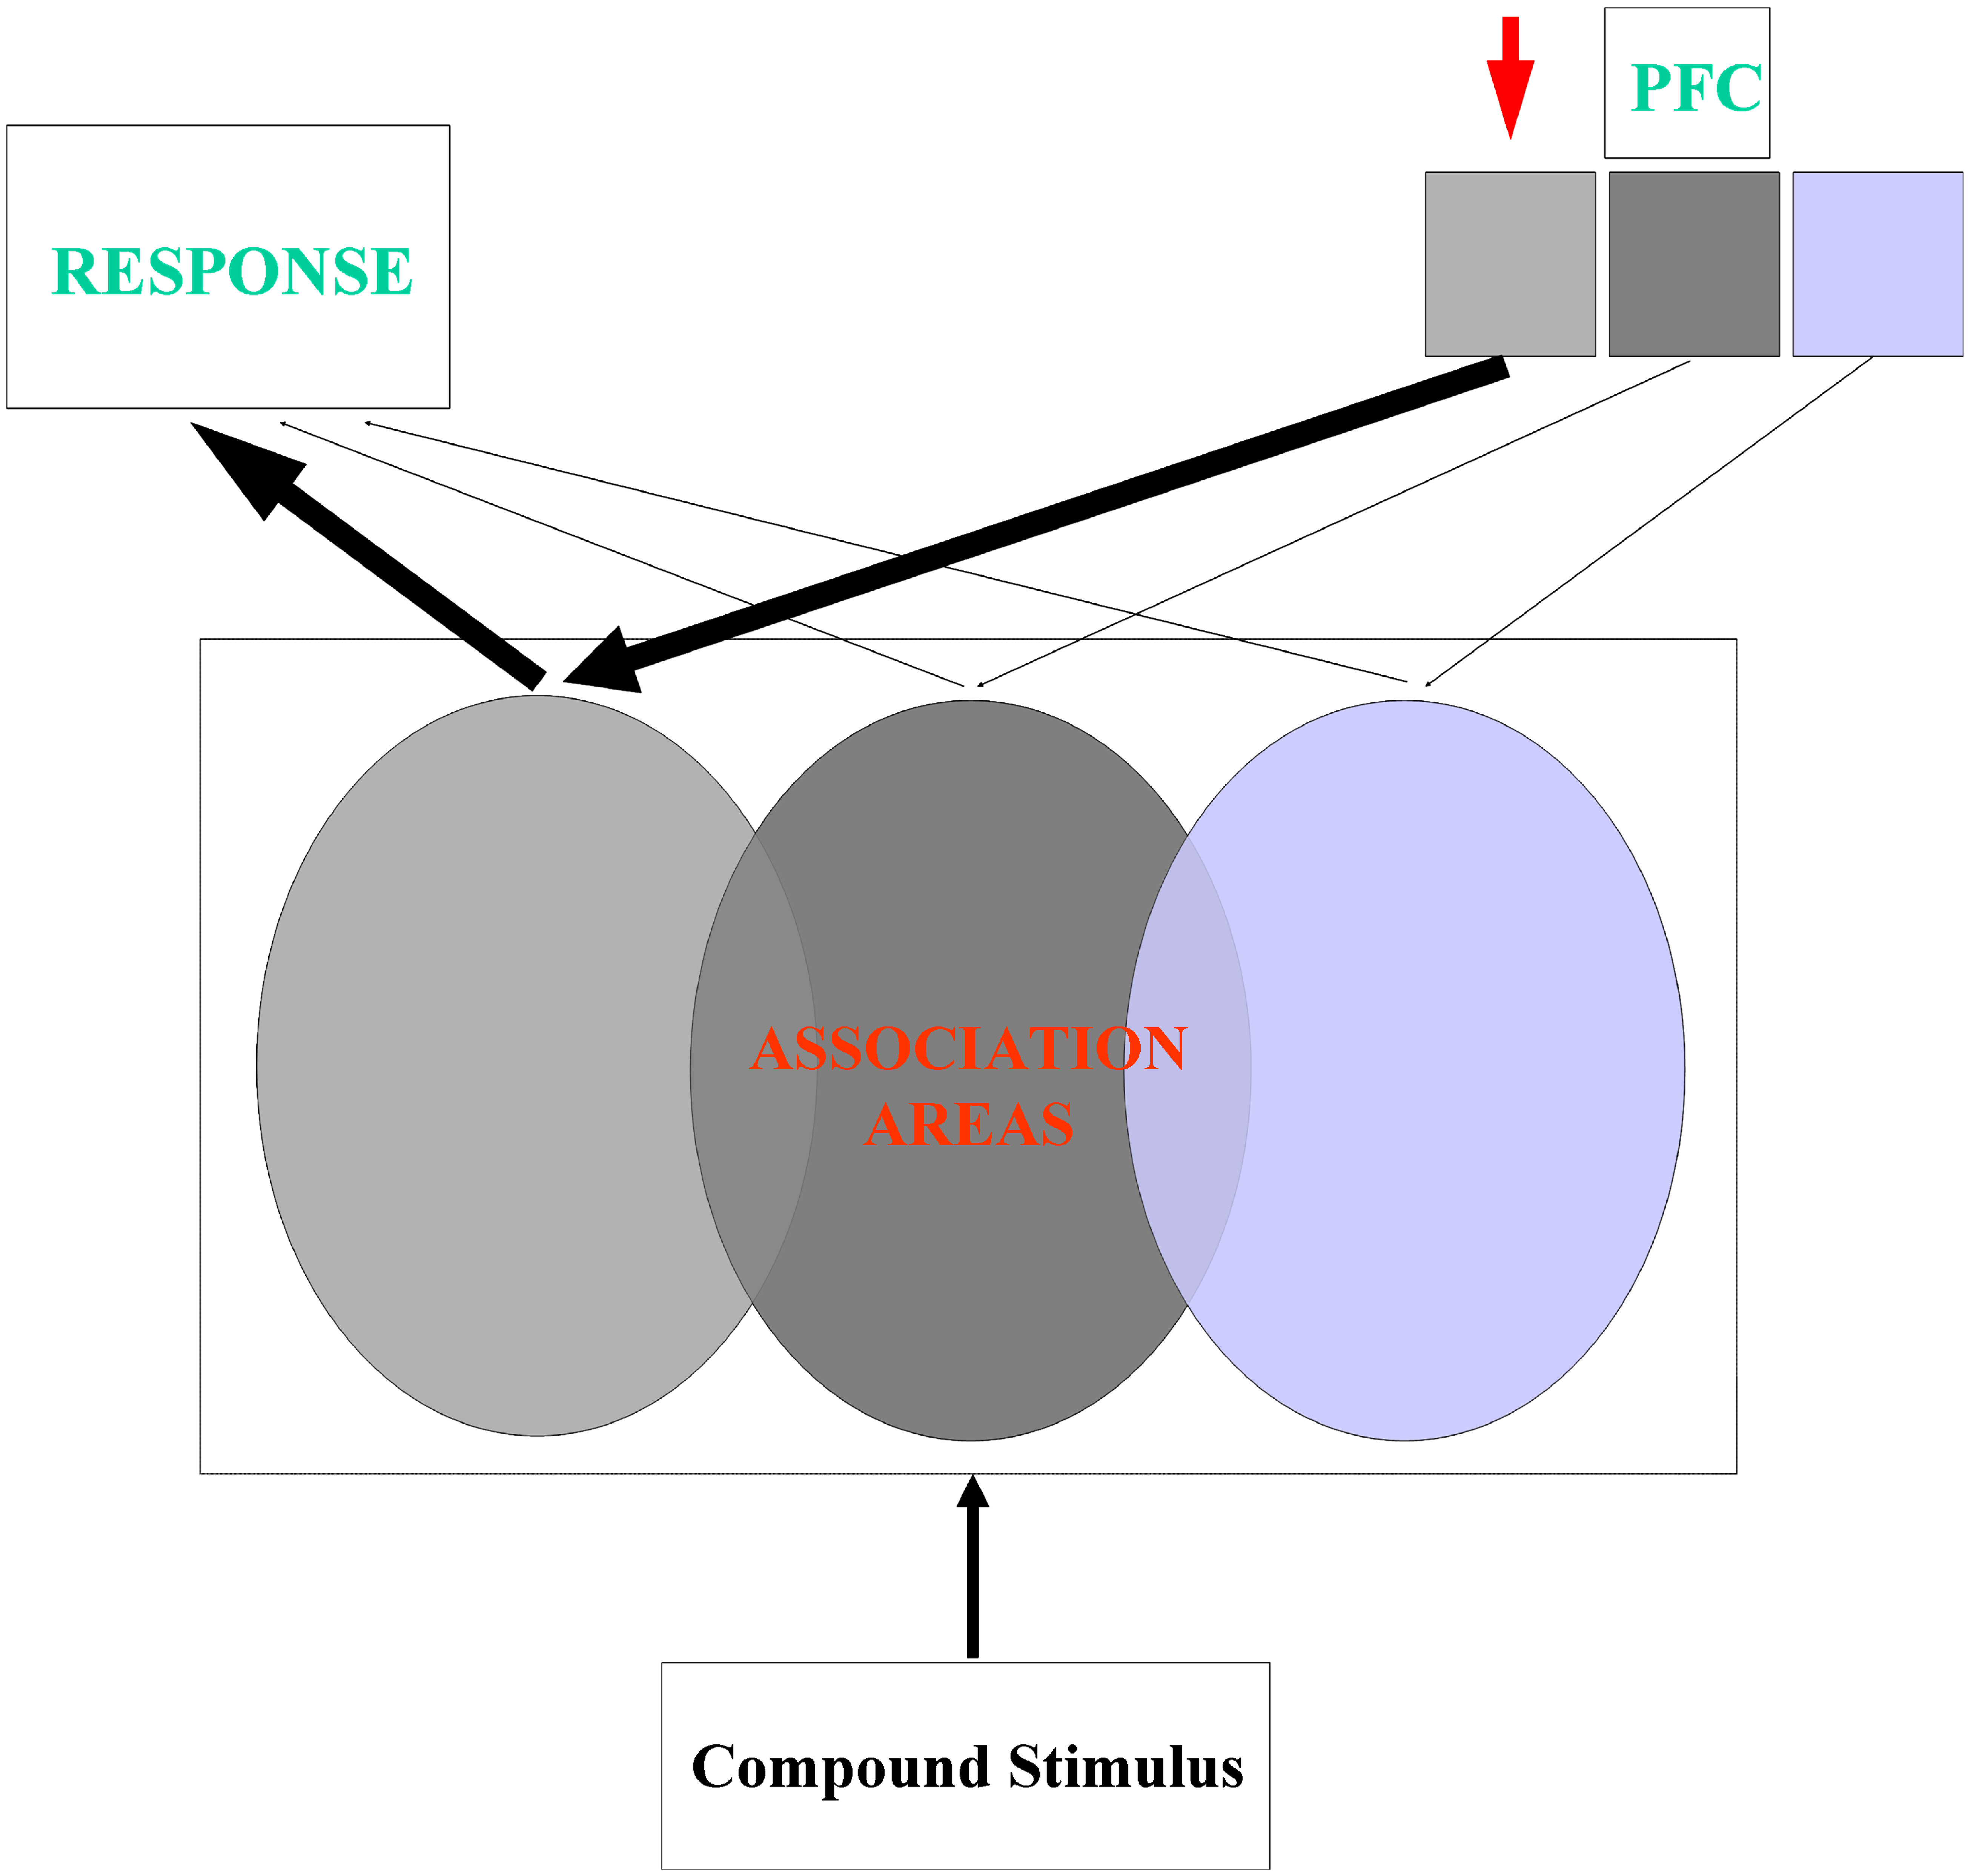
\includegraphics[width=70mm]{figures/so_model_d1_persev_new_2.eps}
\end{center}
\caption{Top panel represents a cartoon model of the stimulus overselectivity task where the PFC is able to flexibly adjust its representations (normal condition).  The resulting ``weights'' driving the response are all similar, resulting in each dimension or feature having equal influence over the response.  The bottom panel represents inflexible updating of the PFC (autism condition).  The red arrow indicates that the PFC is ``stuck'' on the first dimension or feature.  The weights are biased in favor of the feature perseverated on by the PFC, resulting in behavior being dominated by a restricted subset of those available, demonstrating overselectivity when simulating autistic performance.}
\label{OS-Model-Cartoon}
\end{figure} 

%The modeling results presented here suggest that, in people with ASD, overselectivity may be driven largely by a learning process that depends upon the PFC to provide appropriate contextual information in learning stimulus to response mappings.  When the PFC is unable to flexibly and appropriately update its contents, representations in cortical areas downstream from the PFC result which are dominated by an overly restricted, or possibly even irrelevant, subset of features and items from the environment. Results presented here, coupled with past research, provide further support for a theory of perseverative attention to a restricted subset of features in autism.  Indeed, my work provides a plausible mechanism explaining information integration problems in people with ASD.   

\subsection{Summary}
The modeling results presented here suggest that, in people with autism, overselectivity may be driven largely by abnormalities in DA/PFC interactions, causing inflexibility in the shifting of top-down attention.  When the PFC is unable to flexibly and appropriately update its contents, representations in cortical areas downstream from the PFC develop which are dominated by an overly restricted, or possibly even irrelevant, subset of features from the environment.  Poor generalization occurs, under this account, due to the same abnormal cortical representations.  The inability to flexibly update the PFC increases the likelihood that the only environmental associations that will be learned in a given situation will involve spurious correlations (e.g., idiosyncratic features of the training process), with other, more relevant, factors escaping attention.  Subsequent dependence on such spurious correlations can cripple generalization performance.  We suggest that learning over extended developmental timescales with this impairment may lead to behavior which looks like an integration problem on the surface, but, is actually just integrating a limited amount of information.  The results presented here, coupled with the previous research on how DA/PFC impairments can explain executive dysfunction in autism, provide further support for a common neurological cause underlying a variety of behaviors observed in autism.   

